% Generated by Listas/make_statements.py from pratica-lecture-08.md, item 2. Do not edit.
\textbf{Source.} Gibbons (1992), \emph{Game Theory for Applied Economists}, §4.1 Problems, Problem 4.1, p.~245 {[}PDF p.~251{]}. Reproduced verbatim. Answer: none in the book.



\begin{quote}

4.1. In the following extensive-form games, derive the normal-form game and find all the pure-strategy Nash, subgame-perfect, and perfect Bayesian equilibria.



\pandocbounded{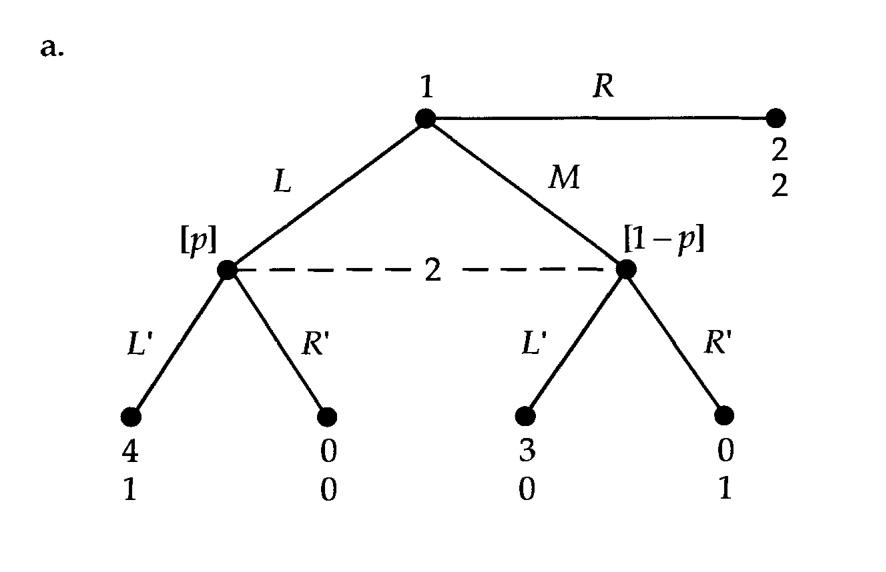
\includegraphics[keepaspectratio,alt={Problem 4.1, game a}]{../figures/gibbons-4-1a.png}}



\pandocbounded{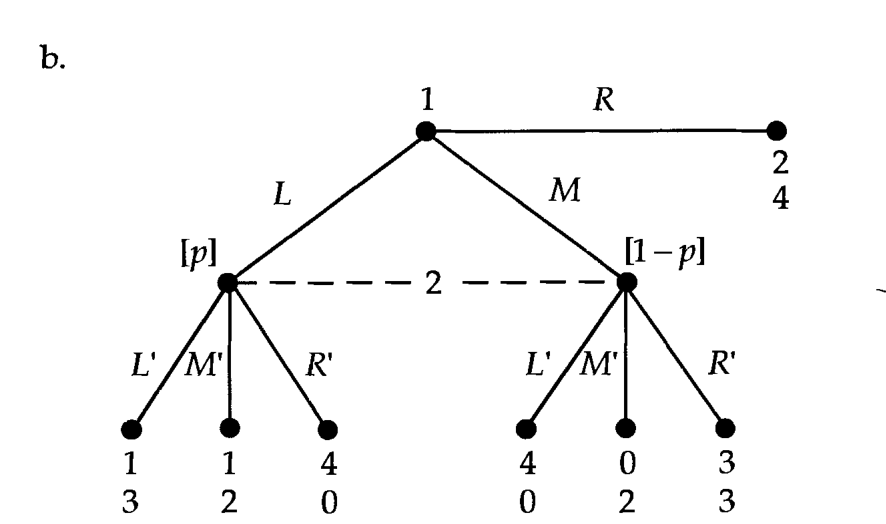
\includegraphics[keepaspectratio,alt={Problem 4.1, game b}]{../figures/gibbons-4-1b.png}}

\end{quote}

